\input{./econtexRoot.texinput}
\documentclass[\econtexRoot/Chp1proposal]{subfiles}
\onlyinsubfile{\externaldocument{\econtexRoot/Chp1proposal}} % Get xrefs -- esp to apndx -- from main file; only works if main file has already been compiled

\begin{document}

\onlyinsubfile{\setcounter{section}{2}}
\section{Model}
\notinsubfile{\label{sec:Model}}

\par My model of labor income risk is standard: it has transitory and permanent shocks calibrated with standard datasets like the PSID. Specifically, household income $(y_t)$ can be expressed as the following:

$$ y_t = p_t \xi_t W_t, $$
where the aggregate wage rate is $(W_t)$, the permanent income component is $(p_t)$, and the transitory shock component is $(\xi_t)$. I assume that the level of permanent income for each household follows a geometric random walk:

$$ p_t = p_{t-1} \psi_{t}, $$
where the white noise permanent shock to income with a mean of one is represented by $\psi_t$.

\par The probability of becoming unemployed is $\mho$; in this case, the agent will receive unemployment insurance payments of $\mu > 0$. With probability $1 - \mho$ the agent is employed and tax payments $\tau_t$ are collected as insurance for periods of unemployment. Altogether, the transitory component of income is given by:

\begin{equation*}
\xi_t =
    \begin{cases}
        \mu & \text{with probability $\mho$,} \\
        (1-\tau_t) l \theta_t & \text{with probability $1-\mho$,}
    \end{cases}
\end{equation*}
where $l$ is the time worked per agent and the parameter $\theta$ captures the white noise component of the transitory shock.

\par Next, I present a standard model of household behavior. The sequence of consumption functions $\{c_{t+n}\}^{\infty}_{n=0}$ associated with a household's optimal choice over a lifetime must satisfy:

\begin{eqnarray*}
  v(m_t) &=& \max_{c_t} u(c_t(m_t)) + \beta \cancel{D} \mathbb{E}_{t}[\psi_{t+1}^{1-\rho}v(m_{t+1})] \\
  &\text{s.t.}& \\
  a_t &=& m_t - c_t(m_t), \\
  k_{t+1} &=& \frac{a_t}{\cancel{D}\psi_{t+1}}, \\
  m_{t+1} &=& (\daleth + r_t)k_{t+1} + \xi_{t+1}, \\
  a_t &\geq& 0,
\end{eqnarray*}
where I denote $a_t$ as assets, $m_t$ as market resources, $k_t$ as capital, and $\daleth = (1 - \delta)$ as the depreciation factor for capital (see \cite{Carroll2019bst} for a theoretical exposition of consumption behavior in the infinite horizon setting). \footnote{Each of the relevant variables have been normalized by the level of permanent income ($c_t = \frac{C_t}{p_t}$, and so on).}

\subsection{Results}
\par To solve and simulate the model, I follow the calibration scheme captured in table \ref{tab:calib1}.
\hypertarget{calibPY}{}
\begin{table}[ht]
  \centering
  \resizebox{0.8\textwidth}{!}{
    \begin{tabular}{cccc}
        \toprule
        Description & Parameter & Value & Source \\
        \midrule
        Time discount factor & $\beta$ & 0.99 & \cite{Den_Haan2010} \\
        CRRA & $\rho$ & 1 & \cite{Den_Haan2010} \\
        Capital share & $\alpha$ & 0.36 & \cite{Den_Haan2010} \\
        Depreciation rate & $\delta$ & 0.025 & \cite{Den_Haan2010} \\
        Time worked per employee & $\ell$ & 1/.09 & \cite{Den_Haan2010} \\
        Capital/output ratio & $\frac{K}{Y}$ & 10.26 & \cite{Den_Haan2010} \\
        Effective interest rate & $r - \delta$ & 0.01 & \cite{Den_Haan2010} \\
        Wage rate & $W$ & 2.37 & \cite{Den_Haan2010} \\
        Unempl. insurance payment & $\mu$ & 0.15 & \cite{Den_Haan2010} \\
        Probability of death & $D$ & 0.00625 & Yields 40-year working life \\
        Variance of $\log \theta_{t,i}$ & $\sigma^{2}_{\theta}$ & 0.010 x 4 & \begin{tabular}[t]{@{}p{5.5cm}@{}} \cite{Carroll1992}, \\ \cite{Carroll2015} \end{tabular} \\
        Variance of $\log \psi_{t,i}$ & $\sigma^{2}_{\psi}$ & 0.010 x 4/11 & \begin{tabular}[t]{@{}p{5.5cm}@{}} \cite{Carroll1992}, \\  \cite{Debacker2013},  \\ \cite{Carroll2015} \end{tabular} \\
        Unemployment rate & $\mho$ & 0.07 & Mean in \cite{Den_Haan2010} \\
        \bottomrule
    \end{tabular}
    }
    \caption{Parameter values (quarterly frequency) for the perpetual youth (infinite horizon) model.}
    \label{tab:calib1}
\end{table}

\unskip

\par The solution of the model with no heterogeneity in returns (the R-point model) is the one which finds the value for the rate of return $\Rfree$ which minimizes the distance between the simulated and empirical wealth shares at the 20th, 40th, 60th, and 80th percentiles. The empirical targets are computed using the 2004 SCF data on household wealth. The estimation procedure finds this optimal value to be $\Rfree = 1.0153$.

\subsubsection{Incorporating heterogeneous returns}

\par As noted above, recent studies by \cite{aflgdmlp20} and \cite{lblcps18} have not only estimated the rate of return on asset holdings but have also uncovered significant heterogeneity across households. Given this motivation, the next estimation (the R-dist model) assumes the existence of multiple types of agents, each earning a distinct rate of return on their assets.

\par I follow closely the procedure outlined by \cite{cstw2017} Specifically, I assume that different types of households have a time preference factor drawn uniformly from the interval $(\grave{\Rfree} - \nabla, \grave{\Rfree} + \nabla)$, where $\nabla$ represents the level of dispersion. Afterward, the model is simulated to estimate the values of both $\grave{\Rfree}$ and $\nabla$ so that the model matches the inequality in the wealth distribution. To achieve this, the following minimization problem is solved:

$$ \{\grave{\Rfree}, \nabla\} = \text{arg}\min_{\Rfree, \nabla} \bigg( \sum_{i=20, 40, 60, 80} (w_{i}(\Rfree, \nabla)-\omega_i )^{2} \bigg)^{\frac{1}{2}} $$

\par subject to the constraint that the aggregate capital-to-output ratio in this model matches that of the perfect foresight setting:

$$ \frac{K}{Y} = \frac{K_{PF}}{Y_{PF}}. $$

\par Note that $w_i$ and $\omega_i$ give the porportion of total aggregate net worth held by the top $i$ percent in the model and in the data, respectively.

\par The estimation procedure finds this optimal values of $\Rfree = 1.0106$ and $\nabla = 0.0112$. The performance of the estimation of both the R-point and R-dist models, measured by their ability to match the SCF data, is compared in figure \ref{fig:PYUnif}.

 \hypertarget{PYUnif}{}
 \begin{figure}[H]
   \centering
    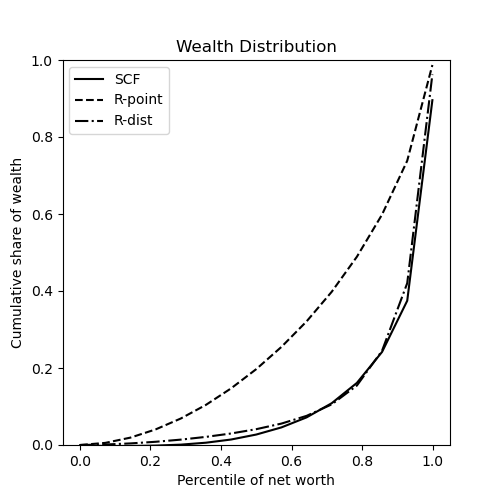
\includegraphics[width=0.7\textwidth]{./Figures/PYUnif.png}
    %
    \caption{Perpetual youth lorenz curve v.s. data}
    \label{fig:PYUnif}
  \end{figure}


\onlyinsubfile{% Allows two (optional) supplements to hard-wired \texname.bib bibfile:
% system.bib is a default bibfile that supplies anything missing elsewhere
% Add-Refs.bib is an override bibfile that supplants anything in \texfile.bib or system.bib
\provideboolean{AddRefsExists}
\provideboolean{systemExists}
\provideboolean{BothExist}
\provideboolean{NeitherExists}
\setboolean{BothExist}{true}
\setboolean{NeitherExists}{true}

\IfFileExists{\econtexRoot/Add-Refs.bib}{
  % then
  \typeout{References in Add-Refs.bib will take precedence over those elsewhere}
  \setboolean{AddRefsExists}{true}
  \setboolean{NeitherExists}{false} % Default is true
}{
  % else
  \setboolean{AddRefsExists}{false} % No added refs exist so defaults will be used
  \setboolean{BothExist}{false}     % Default is that Add-Refs and system.bib both exist
}

% Deal with case where system.bib is found by kpsewhich
\IfFileExists{/usr/local/texlive/texmf-local/bibtex/bib/system.bib}{
  % then
  \typeout{References in system.bib will be used for items not found elsewhere}
  \setboolean{systemExists}{true}
  \setboolean{NeitherExists}{false}
}{
  % else
  \typeout{Found no system database file}
  \setboolean{systemExists}{false}
  \setboolean{BothExist}{false}
}

\ifthenelse{\boolean{showPageHead}}{ %then
  \clearpairofpagestyles % No header for references pages
  }{} % No head has been set to clear

\ifthenelse{\boolean{BothExist}}{
  % then use both
  \typeout{bibliography{\econtexRoot/Add-Refs,\econtexRoot/\texname,system}}
  \bibliography{\econtexRoot/Add-Refs,\econtexRoot/\texname,system}
  % else both do not exist
}{ % maybe neither does?
  \ifthenelse{\boolean{NeitherExists}}{
    \typeout{bibliography{\texname}}
    \bibliography{\texname}}{
    % no -- at least one exists
    \ifthenelse{\boolean{AddRefsExists}}{
      \typeout{bibliography{\econtexRoot/Add-Refs,\econtexRoot/\texname}}
      \bibliography{\econtexRoot/Add-Refs,\econtexRoot/\texname}}{
      \typeout{bibliography{\econtexRoot/\texname,system}}
      \bibliography{        \econtexRoot/\texname,system}}
  } % end of picking the one that exists
} % end of testing whether neither exists
}

\ifthenelse{\boolean{Web}}{}{
  \onlyinsubfile{\captionsetup[figure]{list=no}}
  \onlyinsubfile{\captionsetup[table]{list=no}}
}
\end{document}	\endinput

